\documentclass[11pt,a4paper]{article}
\input{../../sablony/pripravy/priprava.sty}
\usepackage{tikz,pgfplots}
\pgfplotsset{compat=1.18}
\nastavPripravu{1. ročník}{Kvadratické rovnice a nerovnice}{122}{Kvadratické nerovnice I: čtení z grafu}
\begin{document}
\blok{Kvadratické nerovnice I: čtení z grafu}
Znaménko kvadratické funkce na ose $x$ a čtení řešení nerovnice z paraboly.
\begin{definiceBox}[title={Definice - Kvadratická nerovnice}]
\textbf{Kvadratická nerovnice:} například $ax^2+bx+c>0$ nebo $ax^2+bx+c\le0$ pro $a\ne0$.
\end{definiceBox}
\blok{Jaké vztahy můžeme s kvadratickým výrazem zapsat?}
Pro $q(x)=ax^2+bx+c$ ($a\ne0$) rozlišujeme
\[q(x)<0,\quad q(x)>0,\quad q(x)\le0,\quad q(x)\ge0,\quad q(x)\ne0.\]
U $\ne0$ hledáme všechny hodnoty kromě nulových bodů; formálně jde o nerovnost,
ale pro grafické čtení je to jiná otázka než znaménko funkce.
Například $x^2-4\ne0$ má $K=\mathbb R\setminus\{-2;2\}$.
\blok{Metoda a návaznost na graf}
\begin{itemize}
\item Nejdřív načrtni parabolu a zjisti její průsečíky s osou $x$.
\item U ostrých nerovnic nulové body vynechej, u neostrých je zahrň.
\end{itemize}
\blok{Názorné čtení řešení z grafu}
\begin{center}
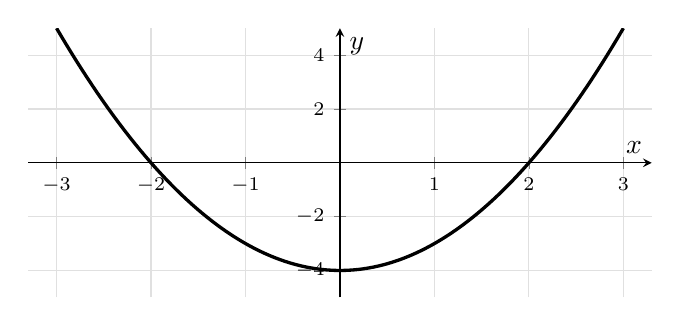
\begin{tikzpicture}
\begin{axis}[width=9.5cm,height=5cm,xmin=-3.3,xmax=3.3,ymin=-5,ymax=5,
axis lines=middle,grid=both,grid style={black!12},minor tick num=0,
xtick={-3,-2,-1,0,1,2,3},ytick={-4,-2,0,2,4},
xlabel={$x$},ylabel={$y$},tick label style={font=\scriptsize}]
\addplot[black,very thick,domain=-3:3,samples=110] {x^2-4};
\end{axis}
\end{tikzpicture}
\end{center}
\poznamka{Na tabuli zvýrazni úsek osy $x$ mezi $-2$ a $2$, kde parabola leží pod osou. To je řešení $x^2-4<0$; při $\le0$ oba krajní body přidáme.}
\blok{Společně řešené příklady}
\begin{prikladReseniBox}[title={Příklad 1}]
$x^{2} - 4<0$
\tcblower
\[
\begin{aligned}
f(x)&=x^{2} - 4\\[2pt]
f(x)=0&\ \Rightarrow\ K_0=\{-2;2\}\\[2pt]
K&=(-2;2)
\end{aligned}
\]
\end{prikladReseniBox}
\begin{prikladReseniBox}[title={Příklad 2}]
$9 - x^{2}\ge0$
\tcblower
\[
\begin{aligned}
f(x)&=9 - x^{2}\\[2pt]
f(x)=0&\ \Rightarrow\ K_0=\{-3;3\}\\[2pt]
K&=\langle-3;3\rangle
\end{aligned}
\]
\end{prikladReseniBox}
\begin{prikladReseniBox}[title={Příklad 3}]
$x^{2} - 4x + 4\le0$
\tcblower
\[
\begin{aligned}
f(x)&=x^{2} - 4x + 4\\[2pt]
f(x)=0&\ \Rightarrow\ K_0=\{2\}\\[2pt]
K&=\{2\}
\end{aligned}
\]
\end{prikladReseniBox}
\blok{Samostatné procvičování}
\begin{zadaniReseniBox}[title={Samostatná práce 1}]
$x^{2} - 5x + 6>0$
\tcblower
\[
\begin{aligned}
f(x)&=x^{2} - 5x + 6\\[2pt]
f(x)=0&\ \Rightarrow\ K_0=\{2;3\}\\[2pt]
K&=(-\infty;2)\cup(3;+\infty)
\end{aligned}
\]
\end{zadaniReseniBox}
\begin{zadaniReseniBox}[title={Samostatná práce 2}]
$- x^{2} + 2x + 3<0$
\tcblower
\[
\begin{aligned}
f(x)&=- x^{2} + 2x + 3\\[2pt]
f(x)=0&\ \Rightarrow\ K_0=\{-1;3\}\\[2pt]
K&=(-\infty;-1)\cup(3;+\infty)
\end{aligned}
\]
\end{zadaniReseniBox}
\blok{Volitelná rezerva}
\poznamka{Studenti si vymyslí obdobný příklad se změnou jednoho koeficientu a vysvětlí, jak se změní počet kořenů či řešení.}
\blok{Domácí úkol}
\begin{zadaniReseniBox}[title={Domácí úkol}]
\begin{enumerate}[label=\alph*),itemsep=2pt]
\item $x^{2} - 9>0$
\item $x^{2} - 3x + 2\le0$
\item $16 - x^{2}\ge0$
\item $x^{2} - 4x + 4>0$
\item $x^{2} + 1<0$
\item $- x^{2} - 4\le0$
\end{enumerate}
\tcblower
\begin{enumerate}[label=\alph*),itemsep=2pt]
\item
\[\begin{aligned}
f(x)&=x^{2} - 9\\[2pt]
f(x)=0&\ \Rightarrow\ K_0=\{-3;3\}\\[2pt]
K&=(-\infty;-3)\cup(3;+\infty)
\end{aligned}\]
\item
\[\begin{aligned}
f(x)&=x^{2} - 3x + 2\\[2pt]
f(x)=0&\ \Rightarrow\ K_0=\{1;2\}\\[2pt]
K&=\langle1;2\rangle
\end{aligned}\]
\item
\[\begin{aligned}
f(x)&=16 - x^{2}\\[2pt]
f(x)=0&\ \Rightarrow\ K_0=\{-4;4\}\\[2pt]
K&=\langle-4;4\rangle
\end{aligned}\]
\item
\[\begin{aligned}
f(x)&=x^{2} - 4x + 4\\[2pt]
f(x)=0&\ \Rightarrow\ K_0=\{2\}\\[2pt]
K&=(-\infty;2)\cup(2;+\infty)
\end{aligned}\]
\item
\[\begin{aligned}
f(x)&=x^{2} + 1\\[2pt]
f(x)=0&\ \Rightarrow\ K_0=\varnothing\\[2pt]
K&=\varnothing
\end{aligned}\]
\item
\[\begin{aligned}
f(x)&=- x^{2} - 4\\[2pt]
f(x)=0&\ \Rightarrow\ K_0=\varnothing\\[2pt]
K&=\mathbb R
\end{aligned}\]
\end{enumerate}
\end{zadaniReseniBox}
\poznamka{Orientační čas: úvod 5 min, společné příklady 18 min, samostatně 15 min, kontrola a shrnutí 7 min. Rezerva je dobrovolná. Číselné parametry modelových aplikací nejsou skutečně naměřená data.}
\end{document}
